%! TEX root = thesis

\chapter{Introduction}

This thesis is a potpourri of some results that span everything from classical mechanics, to statistical mechanics, to quantum mechanics, to engineering.
A common thread that connects these fields is that of asymptotics and geometry.

\begin{figure}
  \begin{center}
    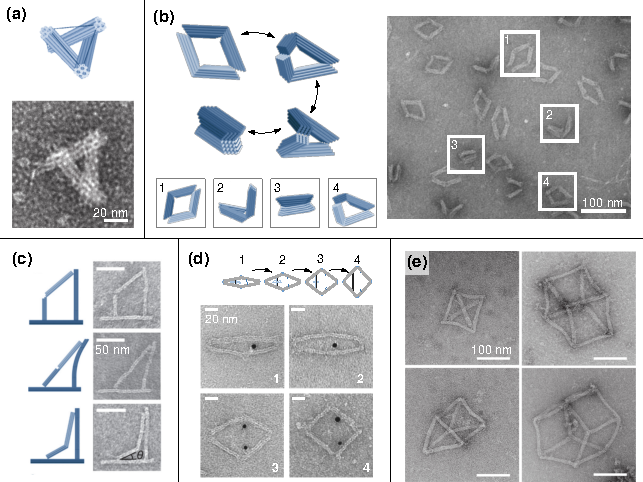
\includegraphics[scale=1.0]{dna.pdf}
  \end{center}
  \caption{DNA origami has been widely used to self assemble a variety of objects at the nanoscale.
    Depicted in the figure are (a) tensegrity structures \cite{liedl2010}; (b), (c) linkage-based mechanisms \cite{marras2015,zhou2015}; (d) a rhombus-shaped nanoactuator~\cite{ke2016}; and (e) self-assembled polyhedra~\cite{iinuma2014}.  All images used with permission.}
  \label{fig:}
\end{figure}

\section{Manifolds}

A manifold, roughly speaking, a set that looks Euclidean\footnote{It is often said that manifolds are smooth sets that look locally ``flat'' and hence can be mapped to an open set in Euclidean space.
This is a bit misleading as the case of the sphere $S^2$ illustrates.
The entire northern hemisphere (except the north pole) of $S^2$ can be mapped to the real plane $\mathbb{R}^{2}$ using stereographic projection.
This means that the two hemispheres of $S^2$ can be covered entirely using two charts.
But neither hemispheres are flat structures.
Flatness also reminds me of curvature, which isn't required for the definition of a smooth manifold, which is much more primitive structure.}

A \emph{regular point} is a point in the domain $X$ where the Jacobian of the map is full rank.
A \emph{regular value} is a point $y \in Y$ such that the Jacobian of all the points in the preimage $f^{-1}(y) \subset X$ is full rank.
Sard's theorem ensures that almost all points in $Y$ are regular values.
%
\begin{theorem}[Sard's theorem]
  The set of critical values of any smooth map $f: X \to Y$, has zero measure in the codomain $Y$.
\end{theorem}

In other words, almost all points in $Y$ are regular values.
As an example, consider $f: \mathbb{R} \to \mathbb{R}$ defined by $x \mapsto x^3 - x$.
The Jacobian in this case is simply the derivative $f'(x) = 3x^2 - 1$, which vanishes only for $x = 3^{-1/2}$.
Hence, every point other than $x = 3^{-1/2}$ is a regular point.%
\footnote{A word of warning is appropriate here: Sard's theorem does not imply that the set of critical points in the domain $X$ is a measure zero subset.
For example, if we consider a constant map, say $f(x) = c \in Y$, then all points in $X$ are critical points.}

One might be tempted to apply the regular value theorem to the energy function itself.
But this wouldn't work since for $E=\|\bm{f}\|^2$ to vanish, $\bm{f}$ must itself vanish, which in turn would make $\nabla E = 2 \bm{f}\nabla\bm{f} = \bm{0}$, making it impossible to apply the regular value theorem on the energy function.

The dimension of tangent space is commonly called a \ac{dof}.

\begin{theorem}[Preimage theorem]
\end{theorem}

\section{Rigidity theory}

\begin{example}[A rank-deficient Jacobian does not always result in a singularity]
  Consider the map $f: \mathbb{R}^{2} \to \mathbb{R}$ defined by $f: (x, y) \mapsto (x^{2} + y^{2})(x^{2} - y)$.
  Since the factor $(x^{2} + y^{2})$ only vanishes at $(x, y) = (0, 0)$, the zero level set $f^{-1}(0)$ is identical to the parabola $y = x^{2}$, which is a smooth manifold.
  However, on this parabola, $\nabla f = [-2x(x^{2} + x^{4}), x^{2} + x^{4}]$, which vanishes at $x = 0$ and is nonzero for all other values of $x$.
Hence, even though $\nabla f$ vanishes at an isolated point, $f^{-1}(0)$ continues to be a smooth manifold.\footnote{Another example where this happens is when $f: (x, y) \mapsto x^{4} - 2x^{2}y - y^{3}$. Again, the gradient $\nabla f$ vanishes at the origin, but the zero level set $f^{-1}(0)$ happens to be a smooth manifold~\cite[Examples 1.1, (vi)]{diesse2020}.}
\altqed
\end{example}

See the notes by \citet{connelly2015} for an introduction to tensegrity structures and the primer by \citet{williams2003} for a slightly advanced treatment.

Forces involved in a state of self stress obey the strong form of Newton's third law and thus cannot possibly result in an unbalanced torque \cite[\S 1.2]{goldstein2002}.
Thus, a tensegrity under self stress is in a state of mechanical equilibrium.
The equilibrium may or may not be stable: again, think of the example with a particle tethered to two walls using springs that are under compression (unstable) or under elongation (stable).

Note that SS exists outside of tensegrity structures.
The only requirement is that all particles interact via central forces.
E.g., one can think of electrostatic analogies, or sticky colloidal clusters.

SS is caused due to linear dependence of constraints.
They might be independent nonlinearly, but on a linear level they are dependent.
Linear constraints are, simply put, hyperplanes.

Maxwell--Calladine theorem is a finite-dimensional toy ``index'' theorem~\cite[\S 2.2]{nakahara2003}.

\subsection{Non-Euclidean origami}

It's easy to understand the configuration manifold of non-Euclidean origami studied by \cite{berry2020}.
A non-Euclidean origami in its ``unfolded'' (or rather, its unactuated) state is not flat.
This means that the linkages forming the origami ``skeleton'' cannot possibly support a self stress since there would be a net unbalanced force in the vertical direction.
Since there can't be a self stress, the Jacobian of the constraint map is full rank everywhere, and thus, the configuration manifold is a smooth 2-dimensional submanifold of $\mathbb{R}^9$ ($M = 7$ and $N = 9$, giving $M - N = 2$).
However, in general, this manifold could be a single connected 2-dimensional manifold or multiple disjoint 2-dimensional manifolds.
If there is positive Gaussian curvature (i.e., an angle deficit) at the center vertex, then the entire structure becomes metastable due to popping up/down of the central vertex.
This popping up and down process is discontinuous and breaks the constraints since the origami has to go through the flat state.
This must be equivalent to having (at least) two 2-dimensional disconnected submanifolds as the configuration space.
When the central vertex has negative Gaussian curvature (i.e., an angle excess), then the origami lacks is metastability.
This must be equivalent to having a single 2-dimensional submanifold as the configuration space.
Note that the manifold can still be disconnected in general, but for the case presenented in \cite{berry2020} it isn't.
What I'm saying is, here there is no reason for the manifold to be connected, but in the previous case (positive Gaussian curvature), it is always disconnected because of physical reasons.
It isn't topology that tells us if the manifolds are disconnected, it's physics.
When there is no Gaussian curvature at the center vertex, the ``unfolded'' state is flat and the origami supports a self stress and the Jacobian drops rank.
This leads to a singularity in the configuration manifold.

\begin{figure}
  \begin{center}
    \includegraphics{zerodof.pdf}
  \end{center}
\caption{A zero \ac{dof} linkage without self stress.  Note how the two constraint manifolds $\mathcal{M}_1$ and $\mathcal{M}_2$ are transverse to each other.}
  \label{fig:hello}
\end{figure}

See the thesis \cite{lengyel2002}.

\begin{figure}
  \begin{center}
    \includegraphics{zerodof_spring.pdf}
  \end{center}
\caption[foo]{A zero \ac{dof} linkage without self stress.  Note how the two constraint manifolds $\mathcal{M}_1$ and $\mathcal{M}_2$ are transverse to each other.}
  \label{fig:hello2}
\end{figure}
\pagebreak

\section{Laplace's method}

To evaluate
%
\begin{equation}
  \int_{a}^{b} \dd{x}\, g(x) e^{-\beta U(x)},
\end{equation}
when $\beta$ is large, we first expand $U(x)$ to $\mathcal{O}(x^{2})$ around a critical point $x_{0}$ with $U'(x_{0}) = 0$.
This turns the above integral into a standard Gaussian integral
%
\begin{equation}
  \int_{a}^{b} \dd{x}\, g(x_{0}) \exp\left\{-\beta\left[U(x_{0}) +  U''(x_{0})(x-x_{0})^{2}\right]\right\},
\end{equation}

\begin{figure}
  % \begin{center}
  %   \includegraphics[scale=1.0]{file}
  % \end{center}
  \caption{Plot of the function $U(x) = 9x^{2} + \sin^{2}{3x} + (1-x)\sin^{2}{6x}$ and $e^{-\beta U(x)}$ in the interval $[-1,1]$ for $\beta = 0.1, 0.2, \ldots, 6.4$.  For larger values of $\beta$ the plot is clearly indistinguishable from that of a Gaussian with a width of $U''(0)$.}
  \label{fig:}
\end{figure}

\subsection{Degenerate case}

\section{Coarea formula}

Jacobian determinants are the corrective factors relating the elements of areas of the domains and images of functions (Morgan's book).

The coarea formula,\footnote{Sometimes the coarea formula is misleadingly written~\cite{hartmann2007,hartmann2007a} with the determinant of $(\nabla\hat{\xi})\trans\nabla\hat{\xi}$ in the denominator.  But the Jacobian $\nabla\hat{\xi}$ does not have full column rank when $m < n$ and the determinant $\det\,(\nabla\hat{\xi})\trans\nabla\hat{\xi}$ vanishes.}
%
\begin{theorem}[Coarea formula]
  Given an integrable function $\phi: \mathbb{R}^n \to \mathbb{R}$ and
  Consider a map $\hat{\xi}: \mathbb{R}^n \to \mathbb{R}^m$ (with $m \leq n$) whose level sets foliate $N \subseteq \mathbb{R}^{n}$ we have
  \begin{equation}
    \begin{aligned}
      \int_{\mathbb{R}^n} \dd{\bm{q}}\, \phi(\bm{q}) &= \int_{\mathbb{R}^m} \dd{\xi}\,\int_{\mathbb{R}^n} \dd{\bm{q}}\, \delta\left[\hat{\xi}(\bm{q}) - \xi\right] \phi(\bm{q})\\
                                                     &= \int_{\mathbb{R}^m} \dd{\xi}\,\int_{\bm{q} \in \hat{\xi}^{-1}(\xi)} \frac{\dd{\Omega(\bm{q})}}{|\det \nabla\hat{\xi}(\nabla\hat{\xi})^\mathsf{T}|^{1/2}} \phi(\bm{q})\,,
    \end{aligned}
  \end{equation}
  where $\dd\Omega(\bm{q})$ is the area element on the level set $\hat{\xi}^{-1}(\xi)$.
\end{theorem}
\begin{proof}
  %
  \begin{equation}
    \begin{aligned}
      \int_{\mathbb{R}^{n}} \dd\bm{q}\,\delta\left[\hat{\xi}(\bm{q}) - \xi\right] \phi(\bm{q}) &=
      \lim_{\alpha \to \infty} \left(\frac{\alpha}{2\pi}\right)^{m} \int_{\mathbb{R}^{n}} \dd\bm{q}\, \exp\left(-\tfrac{1}{2}\alpha\Abs{\hat{\xi}(\bm{q}) - \xi}^{2}\right) \phi(\bm{q})
    \end{aligned}
  \end{equation}
  %
  \qed
\end{proof}

Shape coordinate on a curve can be arclength.  But it's a useless one since it can't be measured experimentally.

Shape space of a triangle is a cone in $\mathbb{R}^{3}$? Joseph Avron's talk at KITP.

Foliation intuitively means that there is a unique hypersurface that passes through each point.

\begin{example}[Integration in polar coordinates]
  As a simple illustration of the coarea formula, consider evaluating the double integral $\int_{\mathbb{R}^{2}} \dd{x}\dd{y}\, \phi(x,y)$, where $\phi(x, y)$ is some integrable function of $(x, y)$.
  The standard polar angle $\theta$ can be computed using the map $\hat{\theta}(x, y) = \tan^{-1}(x, y)$.\footnote{Here $\tan^{-1}(x, y): \mathbb{R}^{2} \setminus \{(0,0)\} \to (-\pi, \pi]$ is the two-argument variant of the inverse tangent, sometimes denoted as $\mathrm{atan2}(y, x)$ in numerical software.  We cannot use $\tan^{-1}(y/x)$ to compute $\theta$ since the range of principal values of $\tan^{-1}(\cdot)$ is conventionally restricted to $(-\pi/2, \pi/2)$.}
  The level set $\hat{\theta}^{-1}(\theta)$ is a straight line starting at the origin (but excluding it) and making an angle of $\theta$ with the positive $x$ axis.
  It is clear that for values of $\theta \in (-\pi, \pi]$, these level sets foliate the entire $\mathbb{R}^{2}$ plane (excluding the origin).
  Choose $\xi = \theta$ and $\hat{\xi}(x, y) = \hat{\theta}(x, y)$ so that
  %
  \begin{equation}
    \int_{\mathbb{R}^{2}} \dd{x}\dd{y}\, \phi(x, y) = \int_{-\pi}^{\pi} \dd\theta\, \int_{\mathbb{R}^{2}} \dd{x}\dd{y}\, \delta[\tan^{-1}(x, y) - \theta] \phi(x, y).
  \end{equation}
  %
  Now, $\nabla\hat{\theta} = \nabla\tan^{-1}(x, y) = (x^{2} + y^{2})^{-1}\begin{pmatrix}-y & x\end{pmatrix}$.
  We can parameterize the points on $\hat{\theta}^{-1}(\theta)$ in terms of $r > 0$ as $(r\cos{\theta}, r\sin{\theta})$.
  Then, $\nabla\hat{\theta} = r^{-1}\begin{pmatrix}-\sin\theta & \cos\theta\end{pmatrix}$ and $\det\,\nabla\hat{\theta}(\nabla\hat{\theta})\trans = r^{-2}$.
  Putting this in the coarea formula and noting that the surface measure on $\hat{\theta}^{-1}(\theta)$ is just $\dd{r}$, we arrive at
  \begin{equation}
    \int_{\mathbb{R}^{2}} \dd{x}\dd{y}\, \phi(x, y) = \int_{-\pi}^{\pi} \dd\theta\, \int_0^{\infty} \dd{r}\, r \phi(r, \theta),
  \end{equation}
  which is the standard double integral of a function expressed in polar coordinates.\footnote{A similar example is discussed in many books on field theory in the context of the Fadeev--Popov method, e.g., the ones by \citet[Section 7.2]{ryder1996} and \citet[Part III.4]{zee2010}.}
  \altqed
\end{example}

Other examples: density of states.  See paper~\cite{gillespie1983}.

\printpagenotes
